% using aastex version 6
\documentclass[onecolumn]{aastex6}
% These are the available options:
%   manuscript  : onecolumn, doublespace, 12pt fonts
%   preprint    : onecolumn, single space, 10pt fonts
%   preprint2   : twocolumn, single space, 10pt fonts
%   twocolumn   : a two column article. Probably not needed, but here just in case.
%   onecolumn   : a one column article; default option.
%   twocolappendix: make 2 column appendix
%   onecolappendix: make 1 column appendix is the default.
%   astrosymb   : Loads Astrosymb font and define \astrocommands.
%   tighten     : Makes baselineskip slightly smaller
%   times       : uses times font instead of the default
%   linenumbers : turn on lineno package.
%   trackchanges : required to see the revision mark up and print output
%   numberedappendix: Labels appendix sections A, B, ... This is the default.
%   appendixfloats: Needed. Resets figure and table counters to zero

%% these can be used in any combination, e.g.
%%
%% \documentclass[twocolumn,twocolappendix,linenumbers,trackchanges]{aastex6}

\usepackage{amsmath}
%% If you want to create your own macros, you can do so
%% using \newcommand. Your macros should appear before
%% the \begin{document} command.

\newcommand{\vdag}{(v)^\dagger}
\newcommand\aastex{AAS\TeX}
\newcommand\latex{La\TeX}
\newcommand\Kepler{\textit{Kepler}}
\newcommand\red{\textcolor{red}}
\newcommand\blue{\textcolor{blue}}
%% You can insert a short comment on the title page using the command below.
\slugcomment{Introductory Outline. \today}
%%
%% If you wish, you may supply running head information, although
%% this information may be modified by the editorial offices.
%%\shorttitle{\aastex sample article}
\shortauthors{Thompson et al.}

\begin{document}
%% You can add a light gray and diagonal water-mark to the first page
%% with this command:
%%\watermark{\today}

\title{Planetary Candidates Observed by \Kepler. VIII.\\
A Fully Automated Catalog Based on Quarters 1 through 17, Data Release 25\\Tuned For High Completeness and Reliability. }

%\author{Susan E. Thompson and others}
% %Authors Names Kept Separately for clarity.
% \AuthorCallLimit=20
% \fullcollaborationName{Kepler Mission Catalog Team}

\author{Susan E. Thompson\altaffilmark{1,2}}
\email{susan.e.thompson@nasa.gov}
\author{Jeffrey L. Coughlin\altaffilmark{2}}
\author{Fergal Mullally\altaffilmark{1,2}}
\author{Jessie L. Christiansen\altaffilmark{3}}
\author{Christopher Burke\altaffilmark{1,2}}
\author{Michael Haas\altaffilmark{1}}
\author{Steve Bryson\altaffilmark{1}}
\author{Natalie Batalha\altaffilmark{1}}
\author{Joe Catanzarite\altaffilmark{1,2}}
\author{Kelsey Hoffmann\altaffilmark{2}}
\author{Jason Rowe}
\author{Douglas Caldwell\altaffilmark{1,2}}
%\altaffiltext{0}{Susan E. Mullally, susan.e.thompson@nasa.gov}
%\altaffiltext{1}{SETI Institute, 189 Bernardo Ave, Mountain View, CA}
%\altaffiltext{2}{NASA Ames Research Center, Moffett Field, CA}
%\altaffiltext{3}{NExScI}

\author{The Rest of the Kepler Team}
%\author{Interpreters of Catalog}
%\author{Created List of TCEs}
%\author{Made Data Available}
%\author{Made mission possible}

\altaffiltext{0}{Susan E. Mullally}
\altaffiltext{1}{NASA Ames Research Center, Moffett Field, CA}
\altaffiltext{2}{SETI Institute, 189 Bernardo Ave, Mountain View, CA}
\altaffiltext{3}{NExScI}

\begin{abstract}
Enlightening words about the purpose of this final Kepler Catalog and how it fits in with the other Kepler Planet Candidate catalogs. Then some details about how many KOIs we added and how many are planet candidates. 
\end{abstract}


\section{Scope}
Overall, the purpose of this paper is to describe how we sifted through the DR25 TCE table and identified the planet candidates, the transiting candidates with significant secondaries, background eclipsing binaries, ephemeris matches and the false alarms. It also needs to describe how we arrive at the reported physical parameters of each planet, so that interesting populations for occurrence rates and follow-up can be identified.  Finally the Completeness and Reliablity of the catalog should be discussed.

Here is a basic outline.
\begin{itemize}
\item Introduction  (Kepler is great blah, blah, KOI catalog blah blah, Cool Discoveries..)

\item A description of the Q1-Q17 DR25 TCEs

\item A description of Injection and Inversion as True Candidates and False Positives.

\item A description of the Robovetter. Summarize the Robovetter, but lean heavily on Coughlin (2016). Discuss why we needed to improve the Robovetter.  Each metric that changed from DR24 Robovetter should be discussed. A list of all minor RoboVetter flags needs to be created and how they relate to the major flags. A discussion of the Robovetter Scores and how they were calculated.

\item A discussion of how the Robovetter metrics were tuned, how were thresholds set? 

\item Evaluate the Completeness of the catalog based on transit injection in MES vs. Period. Also discuss the Confirmed planets and the number that are missed. Give a sense as to where the robovetter is missing planets.

\item Discuss the Effectiveness. Discuss the importance of reliability and how we can use Inversion to get an estimate (a bound?) of the reliability across MES and Period. Also discuss the False Positive table and the number of incorrect dispositions.  Give a sense as to where/when robovetter is ineffective and/or unreliable.

\item Creating the Catalog: Federating to old KOIs, Transit model fits and comparision to DV, how the robovetter was run (inputs/outputs, a summary),  Catalog deliverables. 

\item Analysis of the content of the catalog: Show Candidates on the radius vs. insolation flux labeled by stellar temperature (Coughlin Fig 7.), discuss Multi-planet systems, discuss new individual Rocky-HZ Planet Candidates, enumerate the number of new KOIs of different sizes.

\item Discussion of how to use this catalog to do occurrence rates. i.e. what needs to be considered (Completeness and Reliability, suspicious areas of parameter space, are additional cuts required?), not an actual calculation. Indicate what information will be delivered to NExScI to help with these calculations. 

\item Conclusion 


\end{itemize}

%\textcolor{red}
%{
Items we may want to discuss in the paper but I have decided to leave out.
\begin{itemize}
\item The effectiveness or completeness of the catalog as a function of planetary radius and semi-major axis. (ie derived from fits) 
\item A specific list of confirmed planets that now have a reason to be doubted (if any exist)
\item A comparison to EB catalog
\item Analysis of the injected EBs (secondaries) in terms of effectiveness.
\item Measurement of effectiveness or completeness based on hand vetting.
\item Full analysis of completeness and reliability in terms of insolation flux and planet radius. 
\end{itemize}

Items that do not belong in this paper:
\begin{itemize}
\item An estimate of eta Earth or the occurrence rate for any type of planet.
\item Autovetter Results
\item Discussion of metrics not used by the Robovetter.
\item Complete description of the logic of the Robvetter (i.e. see Coughlin et al.)
\item A list of what was missed that are in other Kepler catalogs (Planet Hunters Catalog, Ojeda short period ones, previous KOI Tables, Confirmed planets.)
\end{itemize}
%}

\section{Introduction}

In 2004 the \Kepler\ space telescope was launched into an earth trailing orbit with the goal of finding evidence of transiting exoplanets \citep{Koch2010}. This was done by monitoring the brightness of over 150,000 stars for four years looking for a small decrease in the brightness of the star caused by a planet passing between the star and the \Kepler\ spacecraft.  Since \Kepler's launch in 2009 it has succeeded in identifying X,XXX planet candidates \citep{Borucki2010,Coughlin20016} and X,XXX confirmed \citep[e.g.][]{FOP?} or validated planets \citep[see most recently][]{Morton2016}. 

Because of the \Kepler\ data, the landscape of known exoplanets has expanded, finding smaller planets in more distant orbits from their host stars.  To highlight a few examples,  \Kepler\ found terrestrial planets as small as Kepler-37b \citep{Barclay2013}, a moon sized planet in a 13.3 day period. \Kepler\ has even found small exoplanets in the habitable zone of their host star, e.g. Kepler-186f \citep{Quintana2014} and Kepler-452b \citep{Jenkins2015}.  The Kepler data has also shown how exoplanets are commonly found in exoplanetary systems. These systems can be compact like the system around Kepler-11, where there are six planets all with periods less than XX days. Also, because of the long continuous data set, exoplanets have been found orbiting binary stars, e.g. Kepler-16\citep{Doyle2011}.


The impact of \Kepler\ on our understanding of exoplanets comes not only from these individual systems, but from the plethora of planets of every type that it has found. Understanding how common different types of exoplanets are around different types of stars will be one of its lasting legacy. \Kepler\ has shown us that most stars have exoplanets and that super-Earth and small planets are more common than their larger cousins \citet{Burke2015}.  


And for each of these unique systems, there are a plethora of exoplanets This plethora of planets \Kepler\ has shown that small planets are common 

\begin{enumerate}
\item What is Kepler and what is its mission?
\item How have we made catalogs in the past and why did we switch to a robovetter. What is the robovetter?
\item Introduce what is new in this paper, hint that the population of TCEs is different and that has created challenges in automatic vetting. Introduce how the goal is to get a sense of the completeness and the reliability of the catalog.
\item Introduce the concepts injection and inversion to test the robovetter.
\item Outline how the Robovetter creates Dispositions and the catalog also includes MCMC fits.
\item Create a road map of what is in this paper?
\end{enumerate}

\section{The Q1--Q17 DR25 TCEs}
\section{OBS TCEs}
\label{tces}
The Threshold Crossing Events, TCEs, are periodic events found in the Kepler time-series data by the Transit Planet Search (TPS) algorithm of the Kepler pipeline \citep[see][]{Twicken2016, Jenkins2017, Fanelli2011}.  The Data Release 25 TCEs were created by running the SOC 9.3 version of TPS on the data release 25, Q1--Q17 \Kepler\ PDC time-series.  For a thorough analysis of the DR25 TCEs and on TPS see \citet{Twicken2016}.  The DR25 TCEs, their ephemerides, and many metrics measured by the pipeline are available at the NASA Exoplanet Archive \citet{Aekeson2013}.  We disposition these signals into planet candidates and false positives.   Because the TCEs act as the input to our catalog, we first describe some of their properties as a whole and reflect on how they are different than the previous TCE table.

There are ??36,xxx DR25 OBS TCEs (Observed TCEs).  We have plotted their distribution in terms of both Period and MES (Multiple Event Statistic, a statistic that is similar to signal-to-noise, see \citep{}), in Figure~\label{f:tces}.  Notice an excessive number of short and long period TCEs, as well as many low MES TCEs.  For comparison, if you will excuse a bit of foreshadowing, the marginalized distribution of our planet candidate catalog is shown in red on the same figure.

\begin{figure*}
 \begin{center}
  \includegraphics[width=\linewidth]{tce-dist.png}
  \caption{\ref{f:tces} A two dimensional histogram of the number of TCEs by Period and MES. A histogram of the number of TCEs by Period are projected along the x-axis and are shown at the top. A histogram of the number of TCEs by MES are projected along the y-axis and are shown on the right. For reference we show the distribution of the DR25 catalog's planet candidates in red on both the marginalized period and MES histograms.
 \end{center}

As with previous TCE catalogs, the short period ($\lt 10$\,d) excess is dominated by true, sinusoidal variability of the star. The long period excess is dominated by instrumental noise. A decrease in flux caused by a cosmic ray hit (a.k.a. SPSD, Sudden Pixel Sensitivity Drop-out), can match-up with natural fluxuations in the data to produce a TCE. Also rolling-band is highly significant on some channels \citep[see p??][]{KDCH} and since the spacecraft rolls every 90\,days, these variations can easily line-up to produce the peak at 370\,d


\end{figure*}



\section{Tools for Evaluating Performance}
 At our disposal we have two additional data sets with which to test our metrics, a population of signals we know to be real (Injection) and a population of signals we know to be false (inversion). We use these to gain a sense of the quality of our catalog.
\subsection{Injection} 
A Quick summary of how injection was done and what we produce with injection. Show a plot of the distribution of recovered injected things in terms of period and MES.
\subsection{Inversion} 
A summary of how inversion was done and what we get from it. Discuss where its limitations as a population of false positives, which ones do we know we are missing. If we have a way of ameliorating this issue, like with season scrambling, discuss that too.

\subsection{Previous Catalogs}In addition we have confirmed planets and confirmed false positives. However, these are not great tests for low MES or long Period.


\section{Vetting Methods and Metrics}

\subsection{Robovetter Overview}
Describe here the idea of not-transit-like and how we look for evidence that the signal is due to an eclipsing binary. Include an updated Figure 2 from the previous paper. Introduce the major flags.
\subsubsection{Using the DR24 Robovetter}
 We applied the DR24 robovetter to the DR25 TCEs. 
 We found that we needed to do better in the following areas.
 Don't forget to cite \citet{Tange2011a}.
 %Words about applying the DR24 robovetter to the DR25 TCEs.
Our first attempt at vetting the DR25 TCE list was done by applying the DR24 Robovetter \citep{Coughlin2016}. To do this, we calculated the metrics described in \citet{Coughlin2016}, such as the LPP Metric, the Marshall Metric, the Model-Shift Uniqueness Test, the Significant Secondary Test, the Centroid Offset and the Ephemeris matching.  We were then able to evaluate the performance of this version of the 
robovetter using the pixel-level transit injection and inversion data. 


Clearly, these results indicate that the TCE population had changed enough to require improvements to the robovetter in order to achieve a highly complete and highly reliability catalog.



\begin{figure*}
\centering
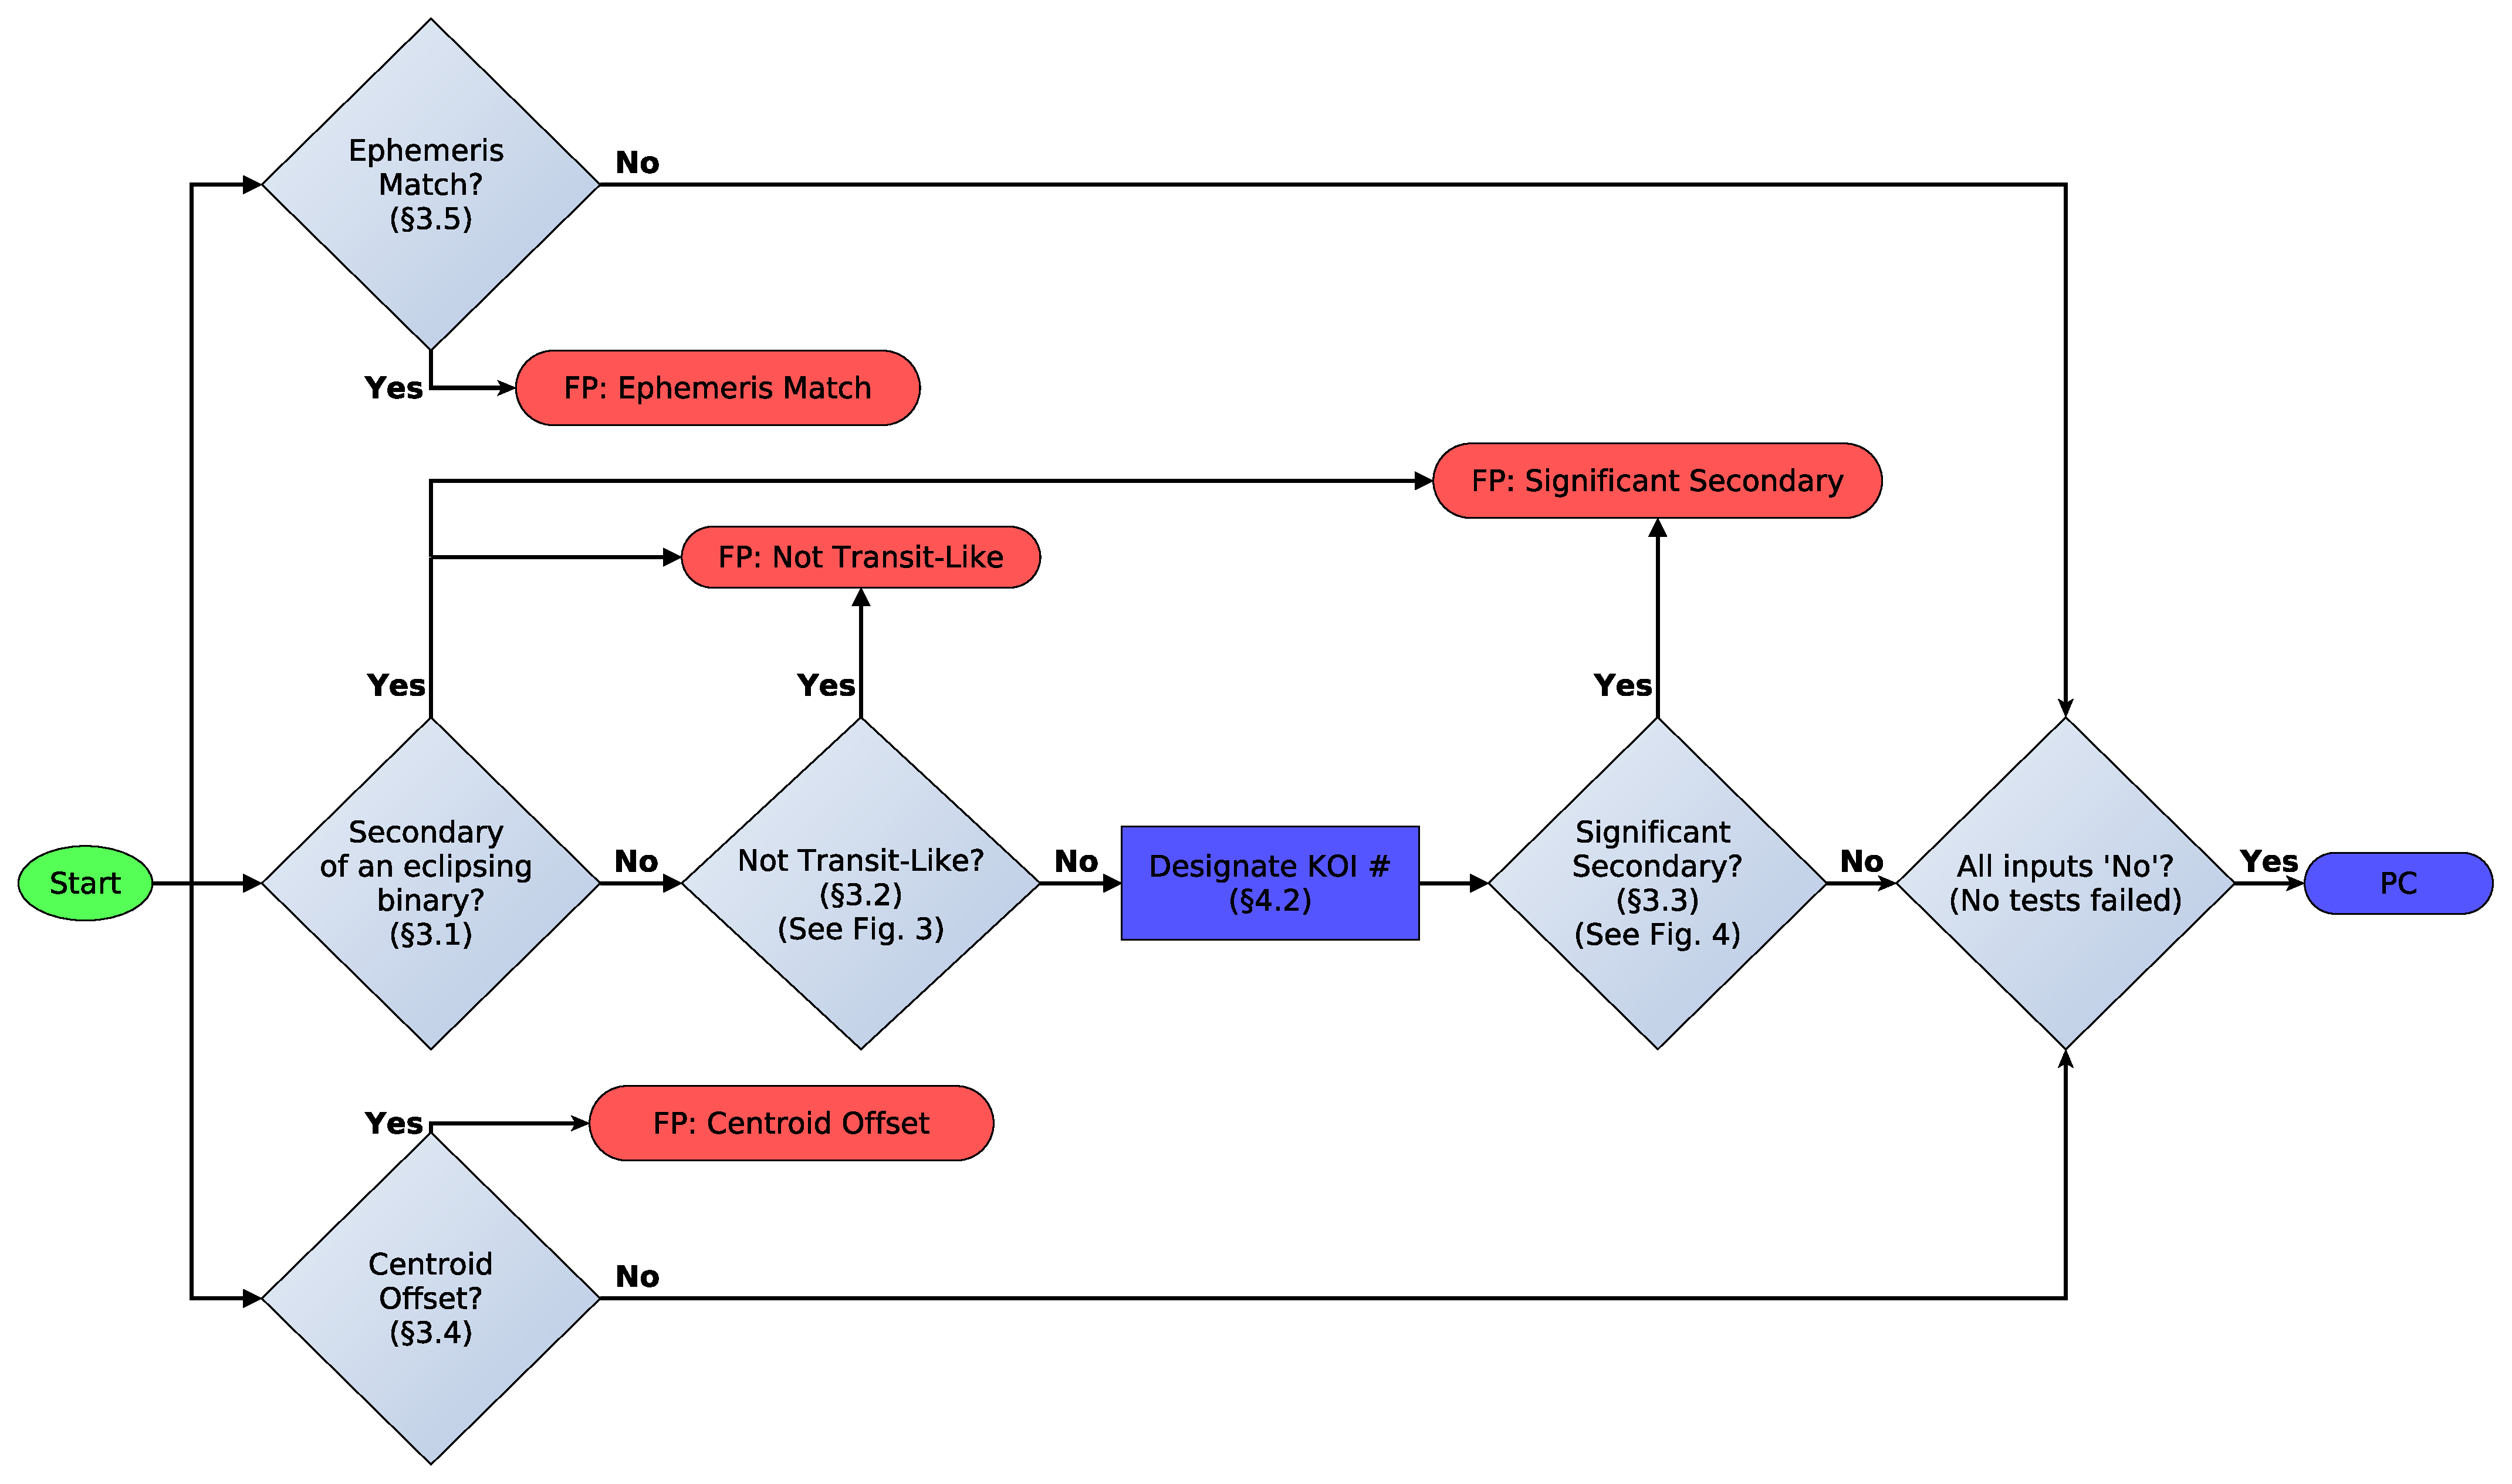
\includegraphics[width=\linewidth]{RoboVetter-Diagram-V3-Overview.pdf}
\caption{\red{An Overview of the Robovetter logic. This is from DR24, so needs to be updated}}
\end{figure*}

\subsection{Individual Metrics, updates and improvements}

\paragraph{Not-Transit-Like Metrics} 
Some metrics that determine if a TCE is not-transit-like operate on the individual transits. We define not-transit-like as anything that does not have three periodic, box- or v-shaped events. Primarily we try to eliminate TCEs caused by instrumental or data-reduction-pipeline effects (like Sudden Pixel Sensitivity Drop Outs or detrending artifacts) and smoothly varying variable stars (pulsators, contact binaries and ellipsoidal binaries) with this high level flag.   These individual metrics are as follows:
\begin{enumerate}
\item Marshall
%%Text describing new Marshall algorithm

\citet{Coughlin2016} used the Marshall method \citep{Mullally16} to identify and reject false alarm TCEs caused by short period transients in the data. Marshall fits the proposed transit with models of a transit and various transients and used a Bayesian Information Criterion to decide which model was the best explanation for the data. Simulations in \citet{Mullally16} showed that Marshall was 95\% complete for TCEs with periods $>150$\,days and correctly rejected 66\% of simulated artifact events. The limit on Marshall's effectiveness at eliminating false alarms was it used a parabola to describe the out-of-transit flux, which failed to capture much of the real observed stellar variability. To ensure high completeness, Marshall was tuned to prevent a variable continuum causing true transits to be rejected, at the cost of a lower than ideal effectiveness.

For this catalog, we use a Gaussian Process approach \citep[GP][]{Rasmussen10} to provide an improved continuum model to improve our effectiveness while maintaining our high completeness. Briefly, our approach aims to model the covariance in the lightcurve to better fit the trends in our data.
A similar approach was used by \citet{ForemanMackey16} to model single transits due to very long period planets ($P > 1000$\,days).

Our procedure is as follows. For each individual proposed transit event, we select a snippet of PDC data 30 times the reported transit duration centred on the event. Where the event happens near the start (or end) of a quarter, we take a snippet of similar length anchored at the start (or end) of the quarter. We use the George package \citep{Ambikasaran14} to fit the covariance of the out-of-transit flux with an exponential squared function, $ {\mathrm{Cov(\delta t})} = A \exp{ (\delta t/\ell)^2}$, where $A$ and $\ell$ are tunable parameters. 

We next fit four models to the entire snippet.

\begin{equation}
\left.\begin{aligned}
G(t | A, \ell) + y_0 \\
G(t | A, \ell) + y_0 + S(t)\\
G(t | A, \ell) + y_0 + S(t)(1 - \exp{\beta t})\\
G(t | A, \ell) + y_0 + S(t - \tau/2) - S(t + \tau/2) 
\end{aligned}\right.
\end{equation}

\noindent
where $G$ is the Gaussian Process model with the tunable parameters held fixed to those found earlier, and $y_0$ is a constant offset. $S(t)$ is given by

\begin{equation}
S(t) = \frac{d}{1 - e^{-\gamma (t-t_0)} }
\end{equation}

\noindent
where $d$ and $t_0$ are tunable parameters, while $\gamma$ is held constant. This function, known as a sigmoid (or logistic) function, has a value of 1 for $t<t_0$, 0 for $t>t_0$, and transitions quickly, but smoothly, between the two states. By using a sigmoid and avoiding the discontinuities in present in the models used by the original Marshall algorithm we can use the L-BFGS-B algorithm \citep{Byrd95} available in the Scipy package \footnote{\url{www.scipy.org}} instead of the less robust Neldar-Mead.

The second function models a discrete jump in the data. We fit this model seeded with a negative-going dip at the predicted time of ingress, and also with a positive-going spike at the predicted egress, as we see both features in \Kepler\ data. The third model fits a Sudden Pixel Sensitivity Drop (SPSD) event, probably caused by a cosmic ray hit on the detection. The last model approximates a box transit. By varying the parameter $\gamma$ we could in principle model transit ingress and egress, but find that extra degree of freedom is not necessary to explain the low signal-to-noise events of most concern.

For each transit the Marshall method returns the BIC score, the preferred model and the difference between the preferred model and the sigmoid box fit.  A transit is considered sufficiently bad when the marshall score exceeds a particular threshold, as with the original Marshall algorithm.  However, in a few cases the Gaussian processes fails, yield extremely large, unbelievable BIC values. In these cases the trasit is set to always pass.  Also, for low MES transits, the expected SES of a transit is sufficiently low that Marshall will be unable to distinguish between the ``no transit" model and a low signal-to-noise transit.  Because of this the robovetter uses the following logic when deciding whether a specific transit is not valid :
\begin{equation}

\end{equation}

{\bf Add some kind of discussion of performance}
{\bf Add link to Source Forge code}
 
\item Skye
\item ChASES
\item Rubble
\item Rocky
\item Grouping single transit failures and recalculating MES and counting the number of transits.
\end{enumerate}

Other metrics operate on data gathered using all the photometric data to determine if the transit signal is transit-like.  These metrics are as follows:

\begin{enumerate}
\item LPP retrained
\item Model Shift Uniqueness
\item SWEET -- for N flag
\item Grouped ChASES
\item Model Shift DMM
\item Model Shift Shape Metric
\item MES/SES

\end{enumerate}

\paragraph{Significant Secondary Metrics}
Some metrics look for evidence that a transit-like signal is actually due to an eclipsing binary (foreground or background).  It primarily looks for evidence of a secondary eclipse, but there are also metrics to look for ellipsoidal

\begin{enumerate}
\item Model Shift Secondary
\item Model Shift Odd-Even
\item Simple Odd-Even
\item SWEET -- for S flag (we might need to combine N and S for this reason)
\end{enumerate}


\paragraph{Centroid Offset} We vet the catalog for evidence that the the target is a false positive because of a background eclipsing binary. The Centroid Robovetter us run on the pixel level data to determine if this is the case.  This is unchanged from the previous two catalogs.  The \textbf{Ghostbuster metric} is also used to determine if the TCE signal is from pixels other than the star.

\paragraph{Ephemeris Matching} We also look for evidence that 


\subsection{Optimization}
How we tuned all the metrics to do the best we can.
Discuss any weaknesses with our methodology.

\section{Evaluate the Dispositions}

\subsection{Catalog Completeness}
\subsubsection{Evaluate recovery of Pixel-level Injected Transits}
\subsubsection{Evaluate recovery of previous KOIs and Confirmed Planets}
\subsubsection{Completeness in Period and MES}

\subsection{Catalog Effectiveness at removing False Positives}
We need a catalog highly effective at removing false positives and false alarms in order to have highly reliable PCs.
\subsubsection{Centroid Robovetter Results for astrophysical FPs}
\subsubsection{Inversion to evaluate Effectiveness for False Alarm removal}
\subsubsection{Evaluate the PC rate of certified FPs}
\subsection{Reliability Estimate}


\section{Putting together the KOI Catalog}
The robovetter vets all TCEs, but we only report those that we consider to be transit-like to the KOI table. We must federate our current list with those KOIs we have made before.
\subsection{Federating to known KOIs}

\subsection{Model Fits using MCMC}

\subsubsection{Comparison between }
\subsection{Deliverables}
We deliver all of the metrics etc..

\section{Overview of the DR25 KOI Catalog}
\subsection{The physical parameters of the planets}
\subsection{New Multi-planet systems}
\subsection{Potentially Rocky Planets in the Habitable Zone}
This is a closer look at some of our most interesting objects.
\subsection{Obvious Problems}

\section{Using This Catalog for Occurrence Rate Calculations}
\subsection{State what the project is providing to make this possible.}


\section{Conclusions}

\acknowledgments
Thanks to GNU parallel \citep{Tange2011a}.

\appendix
\section{List of Acronyms}

\section{Robovetter Minor Flags}
%\section{Robovetter Mnemonic Flags}
\label{minorflagsec}
\red{This needs to be updated with DR25 mnemonic flags.}
In Table~\ref{robodispstab} we list mnemonic flags that describe the results of individual robovetter tests in the comments column. Here we describe the meaning of each flag.

\begin{itemize}
\item[] \textbf{ALT\_ROBO\_ODD\_EVEN\_TEST\_FAIL}: The TCE failed the robovetter's odd-even depth test on the alternate detrending, and thus is marked as a FP due to a significant secondary.
\item[] \textbf{ALT\_SEC\_COULD\_BE\_DUE\_TO\_PLANET}: A significant secondary eclipse was detected in the alternate detrending, but it was determined to possibly be due to planetary reflection and/or thermal emission. While the significant secondary major flag remains set, the TCE is dispositioned as a PC.
\item[] \textbf{ALT\_SEC\_SAME\_DEPTH\_AS\_PRI\_COULD\_BE\_TWICE\_TRUE\_PERIOD}: A significant secondary eclipse was detected in the alternate detrending, but it was determined to be the same depth as the primary within the uncertainties. Thus, the TCE is possibly a PC that was detected at twice the true orbital period. When this flag is set, it acts as an override to other flags such that the significant secondary major flag is not set, and thus the TCE is dispositioned as a PC if no other major flags are set.
\item[] \textbf{ALT\_SIG\_PRI\_MINUS\_SIG\_POS\_TOO\_LOW}: The difference of the primary and positive event significances, computed by the model-shift test using the alternate detrending, is below the threshold $\sigma'_{\rm FA}$. This indicates the primary event is not unique in the phased light curve, and thus the TCE is dispositioned as a FP with the not transit-like major flag set.
\item[] \textbf{ALT\_SIG\_PRI\_MINUS\_SIG\_TER\_TOO\_LOW}: The difference of the primary and tertiary event significances, computed by the model-shift test using the alternate detrending, is below the threshold $\sigma'_{\rm FA}$. This indicates the primary event is not unique in the phased light curve, and thus the TCE is dispositioned as a FP with the not transit-like major flag set.
\item[] \textbf{ALT\_SIG\_PRI\_OVER\_FRED\_TOO\_LOW}: The significance of the primary event divided by the ratio of red noise to white noise in the light curve, computed by the model-shift test using the alternate detrending, is below the threshold $\sigma_{\rm FA}$. This indicates the primary event is not significant compared to the amount of systematic noise in the light curve, and thus the TCE is dispositioned as a FP with the not transit-like major flag set.
\item[] \textbf{CENTROID\_SIGNIF\_UNCERTAIN}: The significance of the centroid offset cannot be measured to high enough precision, and thus the centroid module can not confidently disposition the TCE as a FP. This is typically due to having only a very small number (3 or 4) of offset measurements, all with low SNR.
\item[] \textbf{CLEAR\_APO}: The TCE was marked as a FP due to a centroid offset because the transit occurs on a star that is spatially resolved from the target.
\item[] \textbf{CROWDED\_DIFF}: More than one potential stellar image was found in the difference image. The EYEBALL flag is always set when the CROWDED\_DIFF flag is set.
\item[] \textbf{DV\_ROBO\_ODD\_EVEN\_TEST\_FAIL}: The TCE failed the robovetter's odd-even depth test on the DV detrending, and thus is marked as a FP due to a significant secondary.
\item[] \textbf{DV\_SEC\_COULD\_BE\_DUE\_TO\_PLANET}: A significant secondary eclipse was detected in the DV detrending, but it was determined to possibly be due to planetary reflection and/or thermal emission. While the significant secondary major flag remains set, the TCE is dispositioned as a PC.  
\item[] \textbf{DV\_SEC\_SAME\_DEPTH\_AS\_PRI\_COULD\_BE\_TWICE\_TRUE\_PERIOD}: A significant secondary eclipse was detected in the DV detrending, but it was determined to be the same depth as the primary within the uncertainties. Thus, the TCE is possibly a PC that was detected at twice the true orbital period. When this flag is set, it acts as an override to other flags such that the significant secondary major flag is not set, and thus the TCE is dispositioned as a PC if no other major flags are set.
\item[] \textbf{DV\_SIG\_PRI\_MINUS\_SIG\_POS\_TOO\_LOW}: The difference of the primary and positive event significances, computed by the model-shift test using the DV detrending, is below the threshold $\sigma'_{\rm FA}$. This indicates the primary event is not unique in the phased light curve, and thus the TCE is dispositioned as a FP with the not transit-like major flag set.
\item[] \textbf{DV\_SIG\_PRI\_MINUS\_SIG\_TER\_TOO\_LOW}: The difference of the primary and tertiary event significances, computed by the model-shift test using the DV detrending, is below the threshold $\sigma'_{\rm FA}$. This indicates the primary event is not unique in the phased light curve, and thus the TCE is dispositioned as a FP with the not transit-like major flag set.  
\item[] \textbf{DV\_SIG\_PRI\_OVER\_FRED\_TOO\_LOW}: The significance of the primary event divided by the ratio of red noise to white noise in the light curve, computed by the model-shift test using the DV detrending, is below the threshold $\sigma_{\rm FA}$. This indicates the primary event is not significant compared to the amount of systematic noise in the light curve, and thus the TCE is dispositioned as a FP with the not transit-like major flag set.  
\item[] \textbf{EYEBALL}: The metrics used by the centroid module are very close to the decision boundaries, and thus the centroid disposition of this TCE is uncertain and warrants further scrutiny. No TCEs are marked as a FP due to a centroid offset if this flag is set.
\item[] \textbf{FIT\_FAILED}: The transit was not fit by a model in DV and thus no difference images were created for use by the centroid module. Thus, the TCE is not failed due to a centroid offset by default. This flag is typically set for very deep transits due to eclipsing binaries.
\item[] \textbf{INVERT\_DIFF}: One or more difference images were inverted, meaning the difference image claims the star got brighter during transit. This is usually due to variability of the target star and suggests the difference image should not be trusted. When this flag is set, the TCE is marked as a candidate that requires further scrutiny, i.e., the EYEBALL flag is set and the TCE is not marked as a FP due to a centroid offset.
\item[] \textbf{KIC\_OFFSET}: The centroid module measured the offset distance relative to the star's recorded position in the Kepler Input Catalog (KIC), not the out of transit centroid. The KIC position is less accurate in sparse fields, but more accurate in crowded fields. If this is the only flag set, there is no reason to believe a statistically significant centroid shift is present \citep{Mullally2015c}.
\item[] \textbf{LPP\_ALT\_TOO\_HIGH}: The LPP value \citep{Thompson2015b}, as computed using the alternate detrending, is above the robovetter threshold. This indicates the TCE is not transit-shaped, and thus is dispositioned as a FP with the not transit-like major flag set.
\item[] \textbf{LPP\_DV\_TOO\_HIGH}: The LPP value, as computed using the DV detrending, is above the robovetter threshold. This indicates the TCE is not transit-shaped, and thus is dispositioned as a FP with the not transit-like major flag set.  
\item[] \textbf{MARSHALL\_FAIL}: The TCE failed the Marshall metric \citep{Mullally2015b}, which indicates that the TCE's individual transits are not transit-shaped and more likely due to instrumental artifacts. Thus, the TCE is dispositioned as a FP with the not transit-like major flag set.
\item[] \textbf{OTHER\_TCE\_AT\_SAME\_PERIOD\_DIFF\_EPOCH}: Another TCE on the same target with a higher planet number was found to have the same period as the current TCE, but a significantly different epoch. This indicates the current TCE is an eclipsing binary with the other TCE representing the secondary eclipse. If the ALT\_SEC\_COULD\_BE\_DUE\_TO\_PLANET and DV\_SEC\_COULD\_BE\_DUE\_TO\_PLANET flags are not set, the TCE is dispositioned as a FP with the significant secondary major flag set.
\item[] \textbf{PARENT\_IS\_X}: The TCE has been identified as a FP due to an ephemeris match. This flag indicates the most likely parent, or true physical source of the signal, where X will be substituted for the parent's name. Note that X is not guaranteed to be the true parent, but simply is the most likely source given the information available.
\item[] \textbf{PERIOD\_ALIAS\_IN\_ALT\_DATA\_SEEN\_AT\_X:1}: Using the results of the model-shift test (specifically the phases of the primary, secondary, and tertiary events) a possible period alias is seen at X:1, where X is an integer. This indicates the TCE has likely been detected at a period that is X times longer than the true orbital period. This flag is currently informational only and not used to declare any TCE a FP.
\item[] \textbf{RESID\_OF\_PREV\_TCE}: The TCE has the same period and epoch as a previous transit-like TCE. This indicates the current TCE is simply a residual artifact of the previous TCE after it was removed from the light curve. Thus, the current TCE is dispositioned as a FP with the not transit-like major flag set.
\item[] \textbf{SAME\_P\_AS\_PREV\_NTL\_TCE}: The current TCE has the same period as a previous TCE that was dispositioned as FP with the not transit-like major flag set. This indicates that the current TCE is due to the same not transit-like signal. Thus, the current TCE is dispositioned as a FP with the not transit-like major flag set.
\item[] \textbf{SATURATED}: The star is saturated. The assumptions employed by the centroid robovetter module break down for saturated stars, so the TCE is marked as a candidate requiring further scrutiny, i.e., the EYEBALL flag is set and the TCE is not marked as a FP due to a centroid offset.
\item[] \textbf{SEASONAL\_DEPTH\_DIFFS\_IN\_ALT}: There appears to be a significant difference in the computed TCE depth when using the alternate detrending light curves from different seasons. This indicates significant light contamination is present, usually due to a bright star at the edge of the image, which may or may not be the source of the signal. As it is impossible to determine whether or not the TCE is on-target from this flag alone, it is currently informational only and not used to declare any TCE a FP.
\item[] \textbf{SEASONAL\_DEPTH\_DIFFS\_IN\_DV}: There appears to be a significant difference in the computed TCE depth when using the DV detrending light curves from different seasons. This indicates significant light contamination is present, usually due to a bright star at the edge of the image, which may or may not be the source of the signal. As it is impossible to determine whether or not the TCE is on-target from this flag alone, it is currently informational only and not used to declare any TCE a FP.  
\item[] \textbf{SIG\_SEC\_IN\_ALT\_MODEL\_SHIFT}: The significance of the secondary event divided by the ratio of red noise to white noise in the light curve, computed by the model-shift test using the alternate detrending, is above the threshold $\sigma_{\rm FA}$. Also, the difference between the secondary and tertiary event significances, and the difference between the secondary and positive event significances, both computed by the model-shift test using the alternate detrending, is above the threshold $\sigma'_{\rm FA}$. This indicates that there is a unique and significant secondary event in the light curve, i.e., a secondary eclipse. Thus, assuming the ALT\_SEC\_COULD\_BE\_DUE\_TO\_PLANET flag is not set, the TCE is dispositioned as a FP with the significant secondary flag set.
\item[] \textbf{SIG\_SEC\_IN\_DV\_MODEL\_SHIFT}: The significance of the secondary event divided by the ratio of red noise to white noise in the light curve, computed by the model-shift test using the DV detrending, is above the threshold $\sigma_{\rm FA}$. Also, the difference between the secondary and tertiary event significances, and the difference between the secondary and positive event significances, both computed by the model-shift test using the DV detrending, is above the threshold $\sigma'_{\rm FA}$. This indicates that there is a unique and significant secondary event in the light curve, i.e., a secondary eclipse. Thus, assuming the DV\_SEC\_COULD\_BE\_DUE\_TO\_PLANET flag is not set, the TCE is dispositioned as a FP with the significant secondary flag set.
\item[] \textbf{SIGNIF\_OFFSET}: There is a statistically significant shift in the centroid during transit. This indicates the variability is not due to the target star. Thus, the TCE is dispositioned as a FP with the centroid offset major flag set.
\item[] \textbf{THIS\_TCE\_IS\_A\_SEC}: The TCE is determined to have the same period, but different epoch, as a previous transit-like TCE. This indicates that the current TCE corresponds to the secondary eclipse of an eclipsing binary (or planet if the ALT\_SEC\_COULD\_BE\_DUE\_TO\_PLANET or DV\_SEC\_COULD\_BE\_DUE\_TO\_PLANET flags are set.) Thus, the current TCE is dispositioned as a FP with both the not transit-like and significant secondary major flags set.
\item[] \textbf{TOO\_FEW\_CENTROIDS}: The PRF centroid fit used by the centroid module does not always converge, even in high SNR difference images. This flag is set if centroid offsets are recorded for fewer than 3 high SNR difference images.
\item[] \textbf{TOO\_FEW\_QUARTERS}: Fewer than 3 difference images of sufficiently high SNR are available, and thus very few tests in the centroid module are applicable to the TCE. If this flag is set in conjunction with the CLEAR\_APO flag, the source of the transit may be on a star clearly resolved from the target.
\item[] \textbf{TRANSITS\_NOT\_CONSISTENT}: The TCE had a max\_ses\_in\_mes / mes ratio of greater than 0.9, and a period greater than 90 days. This indicates that the TCE is dominated by a single large event, and thus is due to a systematic feature such as a sudden pixel sensitivity dropout. Thus, the TCE is dispositioned as a FP with the not transit-like major flag set.
\end{itemize}

\bibliographystyle{aasjournal}
\bibliography{References.bib}

\end{document}


